\section{Einführung}
\label{sec:intor}

Die vorliegende Arbeit widmet sich dem Thema der Systemidentifikation mit Hilfe adaptiver Filter.

\begin{figure}[H]
  \centering
  \includegraphics[width=0.5\textwidth]{figures/systemidentifikation.png}
  \caption{Prinzip der Systemidentifikation durch ein adaptives FIR Filter \cite{moschytz2000book}.}
  \label{fig:Systemidentifikation}
\end{figure}

In der Aufgabenstellung \cite{aufgabenstellung} wurden zwei Filtersysteme vorgestellt, ein FIR und ein IIR Filter.
Mit Hilfe der in der Vorlesung besprochenen adaptiven Filter sollen die Koeffizienten der gegebenen Systeme identifiziert werden.
Außerdem werden die Auswirkungen eines Systemwechsels auf die Algorithmen untersucht.
Als Vorbereitung auf die Systemidentifikation wurden der Least-Mean-Square Algorithmus (LMS) und der Recursive-Least-Squares Algorithmus mit Vergessenfaktor (RLS) implementiert.
Die Implementation erfolgte in Python\footnote{Software Repository: \url{https://github.com/Foaly/AdaptiveFilter}} anhand der Rechenvorschrift nach Moschytz \cite{moschytz2000book} (LMS nach S. 85 und RLS nach S. 145).
Anschließend wird noch eine Zeitreihenschätzung mit Hilfe des Kernel Least Mean Squares (KLMS) Verfahren nach der Rechenvorschrift von Weifeng \cite{weifeng2010} (S. 34) implementiert.

\section{FIR-Filter}
\label{sec:fir}

Die erste Aufgabe ist die Systemidentifikation eines FIR Filters mit 5 Koeffizienten.
Das System wird mit Hilfe der LMS und RLS (mit Vergessensfaktor) Algorithmen identifiziert.
Dabei wird der Einfluss durch unterschiedliche Parameter auf das Ergebnis untersucht.
Dazu gehören die Anzahl der Filterkoeffizienten, die Varianz des hinzugefügten Rauschens und die Werte für Schrittweite und Vergessensfaktor.

\begin{figure}[H]
  \centering
      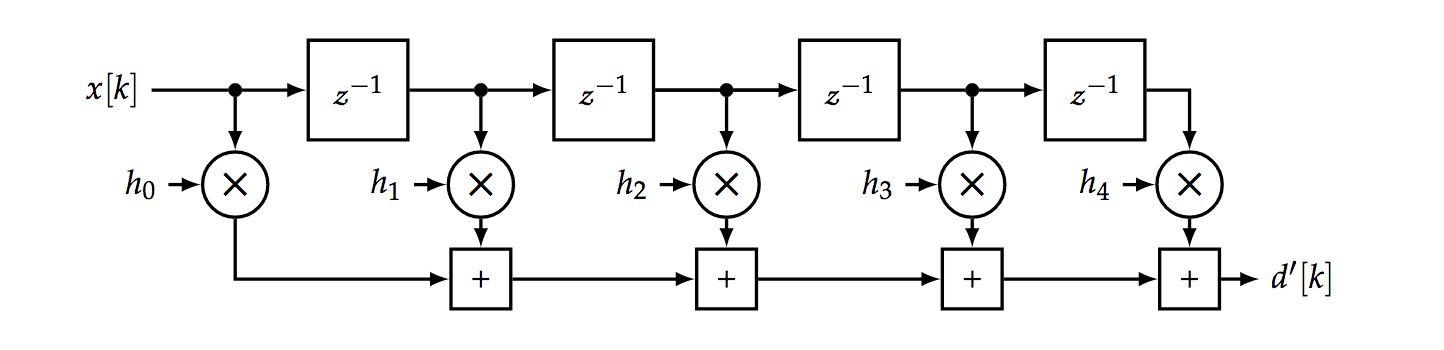
\includegraphics[width=0.9\textwidth]{figures/FIR_System.png}
 \caption{Blockschaltbild des zu untersuchenden FIR Systems (${h_0 = 0.7,}$ ${h_1 = 0.1,}$ ${h_2 = -0.03,}$ ${h_3 = 0.18,}$ ${h_4 = -0.24}$) \cite{aufgabenstellung}.}
	\label{fig:FIR_System}
\end{figure}

In den entstandenen Plots werden die Ergebnisse des LMS und RLS Algorithmus mit Hilfe von je zwei Plots charakterisiert. 
Auf der linken Seite ist der quadratische Fehler (Squared-Error bzw. SE) über den zeitlichen Verlauf in Samplen dargestellt. 
Ein gegen 0 konvergierender Verlauf des Fehlers ist wünschenswert, da dies bedeutet, dass die Differenz zwischen Ausgang des Filters und dem gewünschten Signal kleiner wird und der Algorithmus sein Ergebnis damit selbst verbessert.
Die gestrichelte rote Linie zeigt den Durchschnittswert des Fehlers an, welche es vereinfacht den Wert abzulesen, auf den der Fehler konvergiert.
Außerdem sei angemerkt, dass der Plot des Fehlers mit einem Moving Average von 30 Samplen geglättet wurde, um einzelne Ausreißer zu entfernen und die Lesbarkeit zu erhöhen.
Auf der rechten Seite der Abbildung ist eine Verlaufskurve der durch den Algorithmus gelernten Filterkoeffizienten zu sehen, woraus sich das Adaptionsverhalten des Algorithmus ablesen lässt.
Im Idealfall sollten auch diese je auf einen Wert konvergieren.
Ist dies nicht der Fall, so zeigt dies, dass das Eingangssignal ungeeignet für die Bearbeitung mit diesem Algorithmus ist oder die Einstellung des Algorithmus nicht optimal sind.



\subsection{Anzahl an Filterkoeffizienten}

Die Anzahl der Filterkoeffizienten ist einer der Parameter, der die Systemidentifikation am Stärksten beeinflusst. 
Zu erwarten wäre, dass sich das zu identifizierende System mit weniger Koeffizienten als nötig nicht hinreichend genau abbilden lässt. 
Nach dem Testen verschiedener Mengen an Filterkoeffizienten ($N \in \{1, 2, 5\}$) erwies sich diese Annahme auch als korrekt.
Dabei wird deutlich, dass sowohl dem LMS als auch dem RLS Algorithmus die Approximation mit zu wenig Filterkoeffizienten gleich gut gelingt.
Vergleicht man die Fluktuation in der Fehlerkurve in Abbildungen \ref{fig:N1} und \ref{fig:N2} so wird deutlich, dass diese bei beiden Algorithmen nahezu identisch ist.
Lediglich der Anfang des LMS Algorithmus weißt einen höheren Fehler auf, welcher auf Grund der längeren Konvergenszeit durch die Glättung der Plots nicht so stark beeinflusst wird.
Betrachtet man jedoch den Verlauf der Koeffizient über die Laufzeit der Algorithmen, so fällt auf, dass der LMS länger benötigt bis die Koeffizienten auf einen Wert konvergieren.
Der Koeffizientenverlauf des RLS hat nach Erreichen des Wertes auch ein deutlich stabileres und rauschärmeres Verhalten als die Koeffizienten des LMS.
Dies ist jedoch keine Eingenschaft der Algorithmen als solche, sonder wird durch die Einstellung der Parameter des Vergessensfaktors $\rho$ des RLS und der Schrittweite $\mu$ des LMS bedingt (mehr in Abschnitt \ref{sec:FIR_rho} und \ref{sec:FIR_mu}).
Die unterschiedliche Geschwindigkeit mit der die beiden Algorithmen konvergieren ist ebenfalls darauf zurück zu führen.
Die Legende in Abbildung \ref{fig:N5} zeigt deutlich, dass beide Algorithmen mit der korrekten Anzahl an Koeffizienten auf das identische, korrekte Ergebnis kommen (vgl. mit Abb. \ref{fig:FIR_System}).

\begin{figure}[H]
  \centering
      \includegraphics[width=0.9\textwidth]{{{figures/FIR/N_1_var_0.001}}}
 \caption{Vergleich zwischen LMS und RLS mit je einem Filterkoeffizienten (N=1)}
	\label{fig:N1}
\end{figure}

\begin{figure}[H]
  \centering
      \includegraphics[width=0.9\textwidth]{{{figures/FIR/N_2_var_0.001}}}
 \caption{Vergleich zwischen LMS und RLS mit je zwei Filterkoeffizienten (N=2)}
	\label{fig:N2}
\end{figure}

\begin{figure}[H]
  \centering
      \includegraphics[width=0.9\textwidth]{{{figures/FIR/N_5_var_0.001}}}
 \caption{Vergleich zwischen LMS und RLS mit je fünf Filterkoeffizienten (N=5)}
	\label{fig:N5}
\end{figure}

\subsection{Einfluss der Rauschvarianz}
\label{sec:FIR_sigma}

In der Messstrecke des Systems wird ein AWGN (Additive White Gaussian Noise bzw. Additives Weißes Gausverteiltes Rauschen) hinzugefügt.
Dies ist als $n[k]$ in der schematischen Darstellung \ref{fig:Systemidentifikation} der Messstrecke gekennzeichnet. 
Dadurch lässt sich Testen, welche Algorithmus stabiler und weniger anfällig gegenüber Rauschen ist und sich besser für eine schlechte Übertragungsstrecke einsetzen lässt.
Für die Varianz des Rauschens $\sigma^2$ wurden verschiedene Werte angenommen ($\sigma^2 \in \{0.001, 0.1, 1, 10\}$) und ihr Einfluss auf das Fehlerverhalten der adaptiven Algorithmen untersucht.
Wenig überraschend bedeutet eine Zunahme der Varianz des Rauschen ebenfalls eine Zunahme im quadratischen Fehler und im Adaptionsverhalten der Filterkoeffizienten.
Vergleicht man die Abbildung \ref{fig:N5}, welche mit einem AWGN mit $\sigma^2 = 0.001$ berechnet wurde, mit der Abbildung \ref{fig:sig0.1} ($\sigma^2 = 0.1$) so wird deutlich wie stark das Rauschen die Leistung des adaptiven Filters schwächt.
In Abbildung \ref{fig:N5}, \ref{fig:sig0.1}, \ref{fig:sig1} und \ref{fig:sig10} ist außerdem erkennbar, dass die Filter mit ansteigenden Werten für $\sigma^2$ auf einen jeweils angestiegenen Fehlerwert konvergieren.
In \ref{fig:sig10} mit $\sigma^2 = 10$ ist im Plot des quadratischen Fehlers kein Konvergieren mehr sichtbar.
Bei Betrachten des Verlaufs der Koeffizienten mit verschiedenen Werten für $\sigma^2$ fällt erneut auf, dass der RLS im Vergleich zum LMS eine stärke Toleranz gegenüber Rauscheinflüssen aufweist.
Ebenfalls auffällig ist die deutliche Ähnlichkeit der beiden Fehlerkurven der unterschiedlichen Algorithmen in Abbildung \ref{fig:sig10}.
Dies lässt darauf schließen, dass der Signal-Rausch-Abstand (SNR) so gering ist, dass das Rauschen das eigentliche Signal nahezu komplett überdeckt.

\begin{figure}[H]
  \centering
      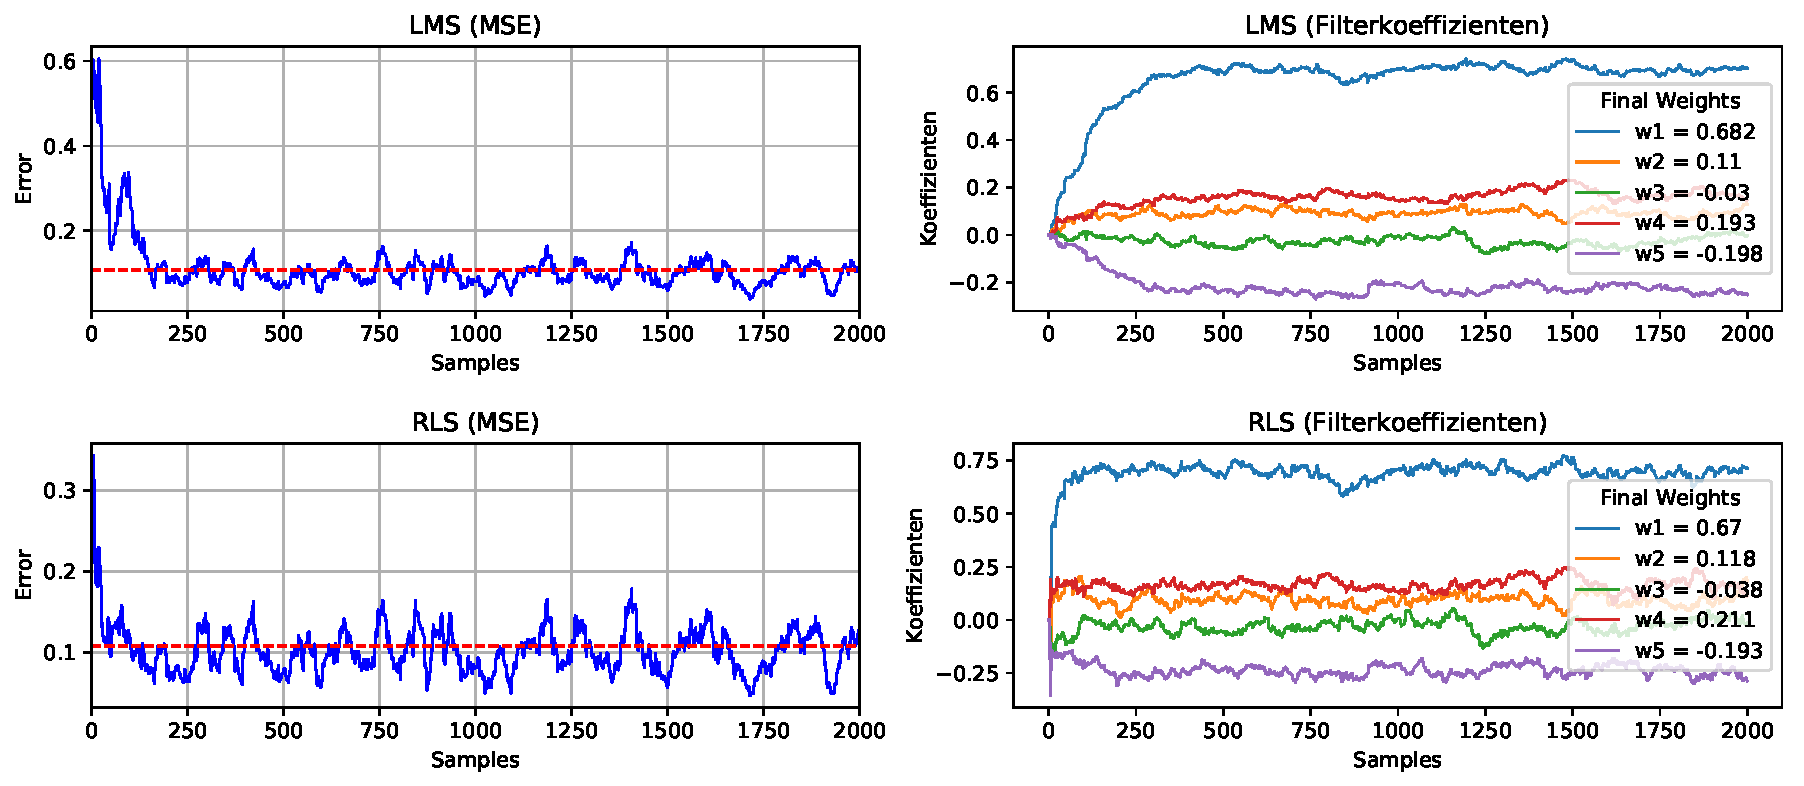
\includegraphics[width=0.9\textwidth]{{{figures/FIR/N_5_var_0.1}}}
 \caption{Vergleich zwischen LMS und RLS bei einem AWGN von $\sigma^2 = 0.1$  (N=5)}
	\label{fig:sig0.1}
\end{figure}

\begin{figure}[H]
  \centering
      \includegraphics[width=0.9\textwidth]{{{figures/FIR/N_5_var_1.0}}}
 \caption{Vergleich zwischen LMS und RLS bei einem AWGN von $\sigma^2 = 1$  (N=5)}
	\label{fig:sig1}
\end{figure}

\begin{figure}[H]
  \centering
      \includegraphics[width=0.9\textwidth]{{{figures/FIR/N_5_var_10.0}}}
 \caption{Vergleich zwischen LMS und RLS bei einem AWGN von $\sigma^2 = 10$  (N=5)}
	\label{fig:sig10}
\end{figure}


\subsection{Einfluss des Vergessensfaktors \boldmath{$\rho$}}
\label{sec:FIR_rho}

Der Vergessensfaktor $\rho$ ist ein Parameter des RLS Algorithmus und liegt im Wertebereich $0 < \rho \leq 1$.
Er dient als Faktor, der bestimmt wie stark in der Vergangenheit zurückliegende Werte gewichtet werden.
Ein Vegessensfaktor von 1 bedeutet, dass alle bisherigen Werte in die Berechnung mit einbezogen werden.
Ist der Wert von $\rho$ sehr gering, so wird nur ein kleiner Teil der am Kürzesten zurückliegenden Werte berücksichtigt.
Während ein hoher Wert dazu führt, dass der RLS Algorithmus sich schlecht an ein sich veränderndes System anpassen kann (siehe Abschnitt \ref{sec:Systemwechsel} Systemwechsel), führt ein zu niedriger Wert zu Stabilitätsproblemen, da nie genug Werte miteinbezogen werden, um das System zu identifizieren.
Betrachtet man die Abbildungen \ref{fig:rho_vergleich} so wird dies ebenfalls deutlich.
Ein niedrigerer Wert für $\rho$ führt zu einem höheren quadratischen Fehler und einem deutlich sprunghaftem und rauschhaften Adaptionsverhalten der Filterkoeffizienten.
Laut Moschytz \cite{moschytz2000book} (S. 145) liegt der Wert für den Vergessensfaktor typischerweise zwischen $0.95 < \rho < 1$.
Bei den bisher abgebildeten Plots \ref{fig:N1} bis \ref{fig:sig10} wurde jeweils ein Vergessensfaktor $\rho = 0.99$ verwendet.

\begin{figure}[H]
  \centering
      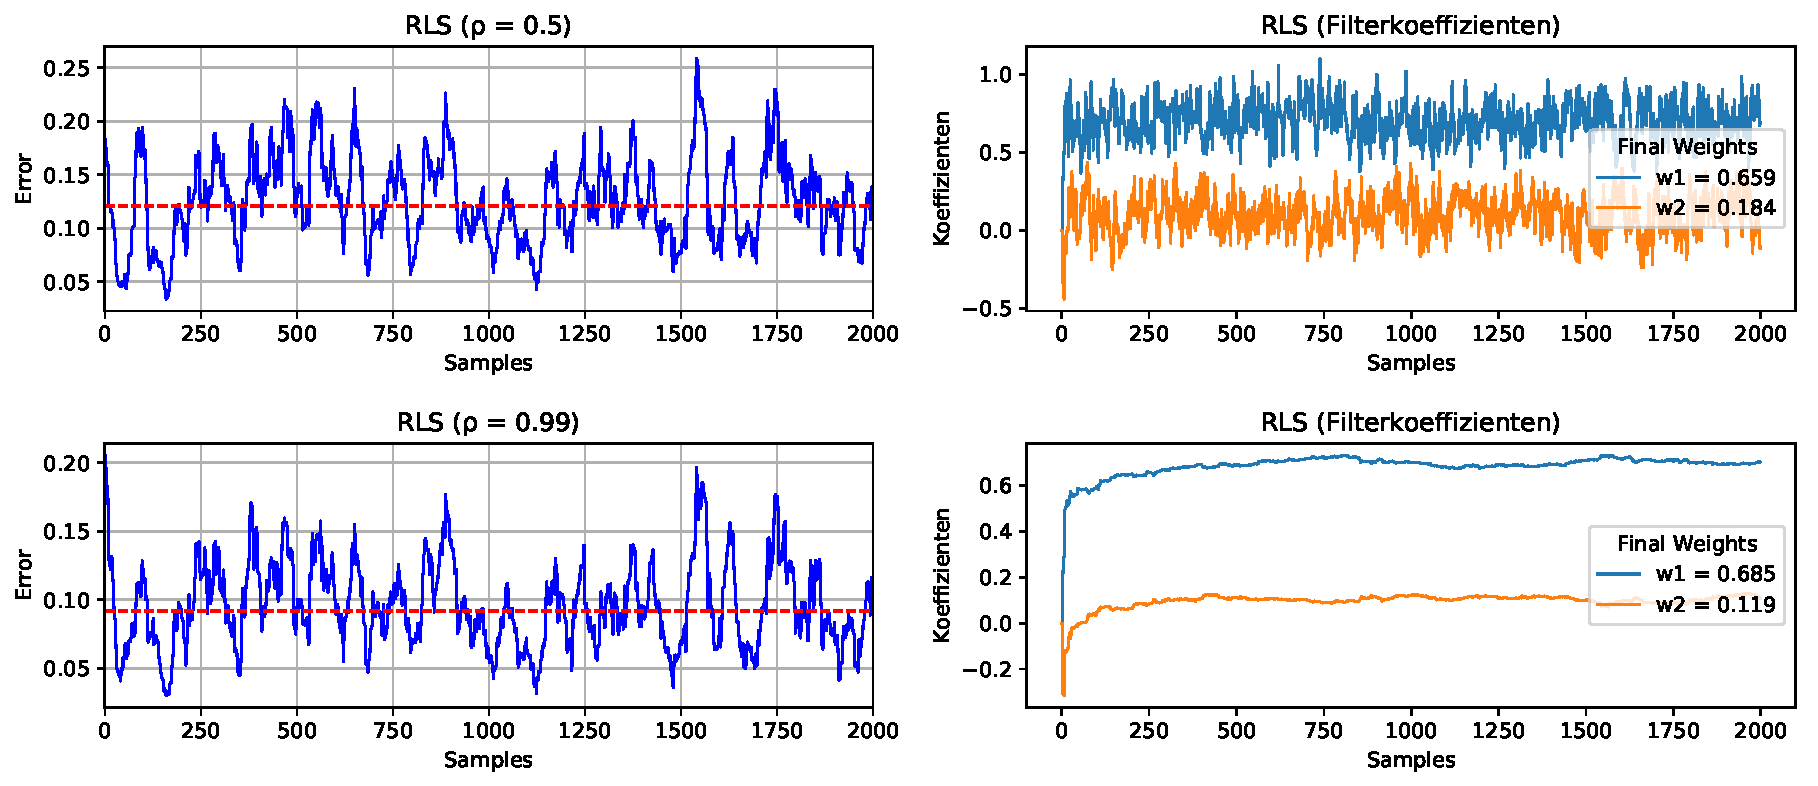
\includegraphics[width=0.9\textwidth]{{{figures/FIR/N_2_var_0.001_rho_vergleich}}}
 \caption{Vergleich zwischen verschiedenen Werten für $\rho$ des RLS ($\rho = 0.5$ oben und $\rho = 0.99$ unten) }
	\label{fig:rho_vergleich}
\end{figure}



\subsection{Einfluss des Schrittweite \boldmath{$\mu$}}
\label{sec:FIR_mu}

Die Schrittweite $\mu$ ist ein Parameter des LMS Algorithmus.
Er kann Werte zwischen $0 < \mu \leq 1$ annehmen und ist ein Faktor der bei jeder Iteration den Fehler $e[n] = d[n] - y[n]$ gewichtet.
Dadurch lässt sich die Geschwindigkeit der Adaption des Algorithmus einstellen.
Ein hoher Wert lässt den Fehler schneller konvergieren, kann allerdings dazu führen, dass das optimal Fehlerminimum nicht erreicht werden kann und dieses in jeder Iteration über- bzw. unterschritten wird.
In den Abbildungen \ref{fig:mu0.01} bis \ref{fig:mu0.2} ist dies mit Hilfe verschiedener Werte für $\mu$ beispielhaft dargestellt ($N=5, \sigma^2=0.01$).
In Abbildung \ref{fig:mu0.01} ist $\mu = 0.001$ was zu einer vergleichsweise langsamen An­nä­herung des Fehlers an den Wert 0 führt, welcher aber erreicht wird.
Wird, wie in Abbildung \ref{fig:mu0.1}, $\mu = 0.1$ gesetzt konvergiert der Fehler zwar schneller, aber erreicht 0 nie ganz (siehe rote gestrichelte Linie für den Durchschnitt) und oszilliert leicht um diesen Wert.
Ein noch höherer Wert, wie $\mu = 0.2$ verdeutlicht das Über- und Unterschreiten des optimalen Fehlerminimums deutlich (siehe \ref{fig:mu0.2})
Die bisherigen Plots \ref{fig:N1} bis \ref{fig:sig10} wurden mit einer Schrittweite von $\mu = 0.01$ erzeugt.


\begin{figure}[H]
  \centering
      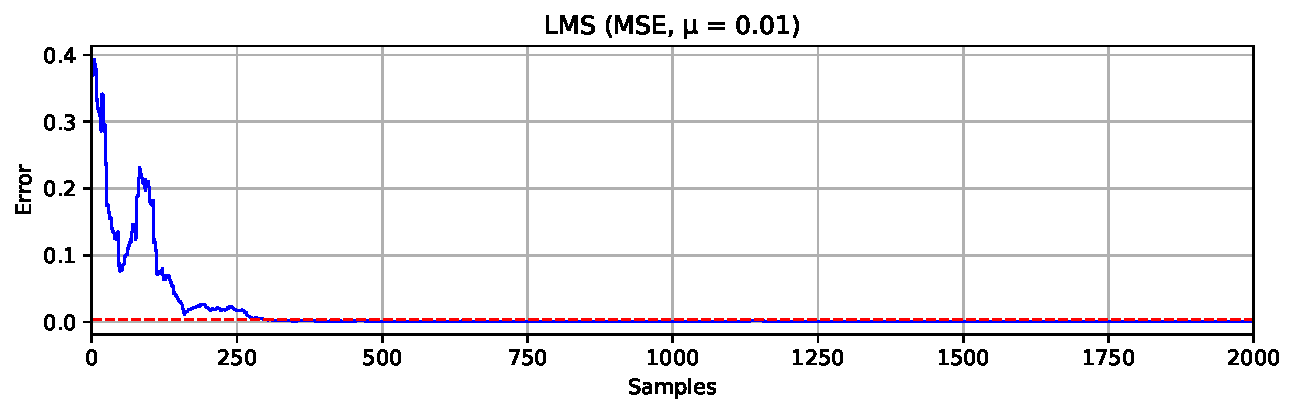
\includegraphics[width=0.7\textwidth]{{{figures/FIR/lms_N_5_var_0.001_mu_0.01}}}
 \caption{LMS mit einer Schrittweite $\mu = 0.01$}
	\label{fig:mu0.01}
\end{figure}

\begin{figure}[H]
  \centering
      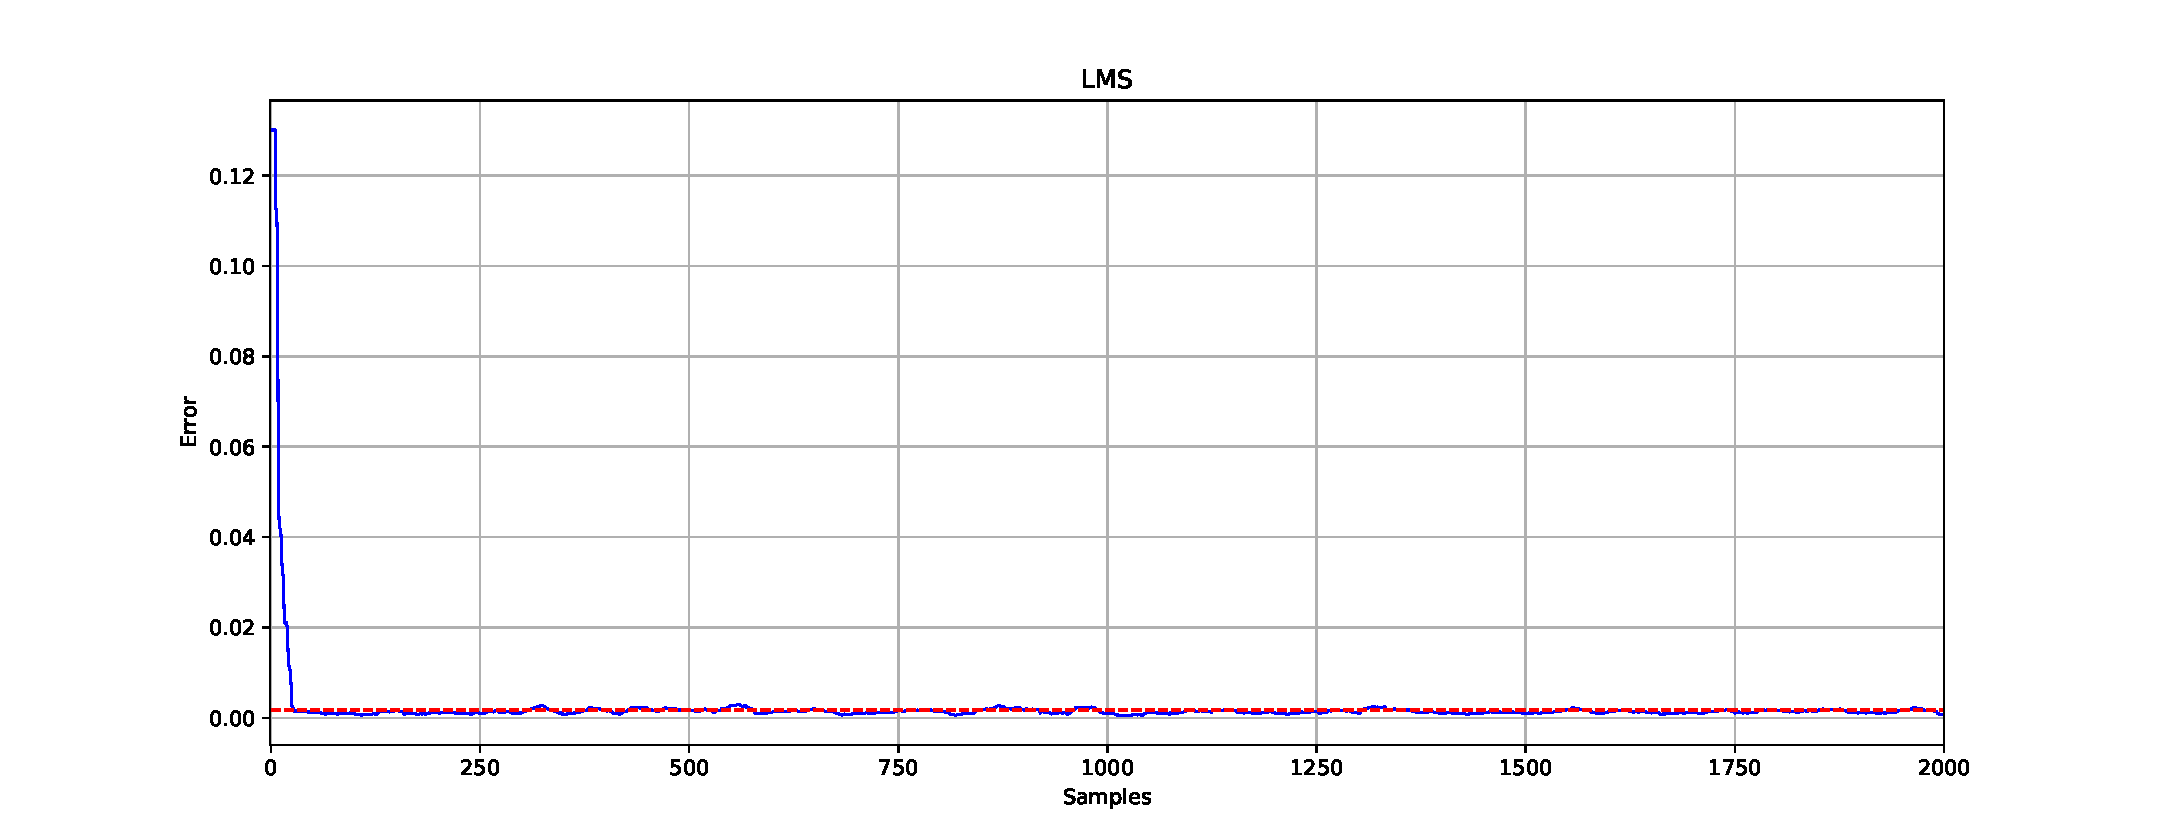
\includegraphics[width=0.7\textwidth]{{{figures/FIR/lms_N_5_var_0.001_mu_0.1}}}
 \caption{LMS mit einer Schrittweite $\mu = 0.1$}
	\label{fig:mu0.1}
\end{figure}

\begin{figure}[H]
  \centering
      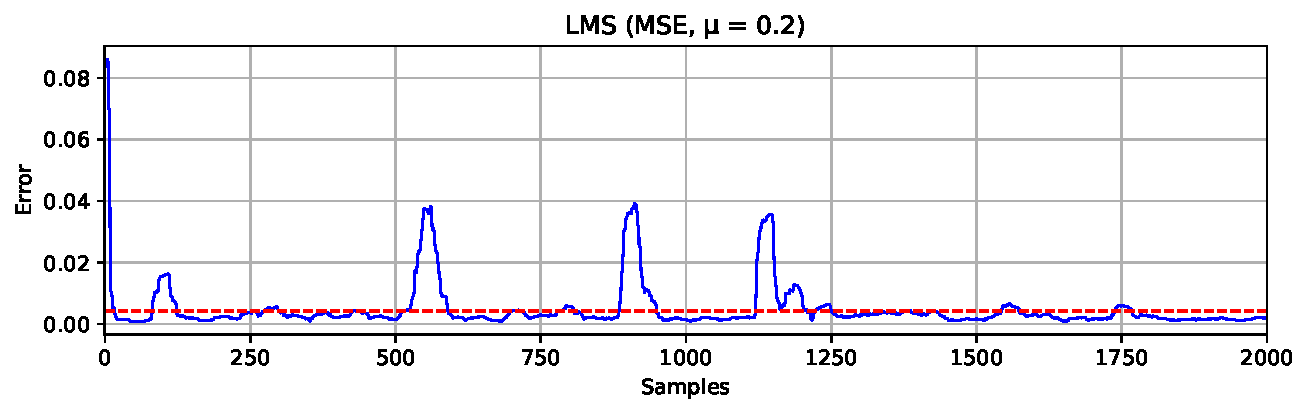
\includegraphics[width=0.7\textwidth]{{{figures/FIR/lms_N_5_var_0.001_mu_0.2}}}
 \caption{LMS mit einer Schrittweite $\mu = 0.2$}
	\label{fig:mu0.2}
\end{figure}



\subsection{Wahl des Lernalgorithmus}

Betrachtet man zunächst nur den Code der beiden Algorithmen so wird deutlich, dass die Algorithmen ein unterschiedliche Komplexität und eine daraus resultierende unterschiedliche Laufzeiten haben.
Der RLS weist dabei eine höhere Komplexität und Laufzeit auf als der LMS.

Außerdem unterscheiden sich die beiden Algorithmen in ihrer Konvergenzzeit der Filterkoeffizienten.
In den oben betrachteten Abbildungen konvergieren die Filterkoeffizienten des RLS schneller als die des LMS, selbst bei einem größeren Wert für die Schrittweite $\mu$ des LMS.
Der Grund dafür liegt in der Architektur der Algorithmen selbst.
Der LMS berücksichtigt bei jeder Interation seiner Adaption jeweils nur die letzten $N$ Werte.
Der RLS hingegen bezieht durch das Aufdatieren der inversen deterministischen Autokorellationsmatrix alle bisherigen Werte, gewichtet durch einen Vergessenfaktor, mit in die Berechnung ein.
Dies führt zur Beobachteten schnelleren Konvergenzzeit des RLS.
Durch das Wählen einer entsprechende Schrittweite lassen sich beim LMS zwar ähnlich schnelle Konvergenzzeiten der Filterkoeffizienten erreichen, allerdings führt dies zu sehr verrauschten und stark schwankenden Filterkoeffizienten, da der LMS durch die größere Schrittweite die Optimalwerte ständig über- und unterschreitet.
Durch das Einbeziehen aller bisheriger Werte erziehlt der RLS wesentlich stabilere Filterkoeffizienten.
Auch das hinzugefügte AWGS stört aus diesem Grund den Verlauf der Filterkoeffizienten des RLS nicht so stark wie die des LMS.
Da es sich bei dem vorliegenden Signal um einen stationären, stochastischen Prozess handelt spielt der Vergessenfaktor $\rho$ des RLS für die Konvergenzzeit noch keine Rolle.

Auf Grund der Eigenschaften des Prozesses liefern beide Algorithmen bei der entsprechenden Wahl der Parameter sehr ähnliche Ergebnisse.







\section{IIR-Filter}
\label{sec:iir}

Das zweite System das untersucht werden soll ist ein IIR Filter mit 2 Filterkoeffizienten.
Bei der Systemidentifikation wird hier analog zu Abschnitt \ref{sec:fir} vorgegangen und die Ergebnisse des LMS und RLS Algorithmus unter Einfluss unterschiedlicher Parameter untersucht.

\begin{figure}[H]
  \centering
      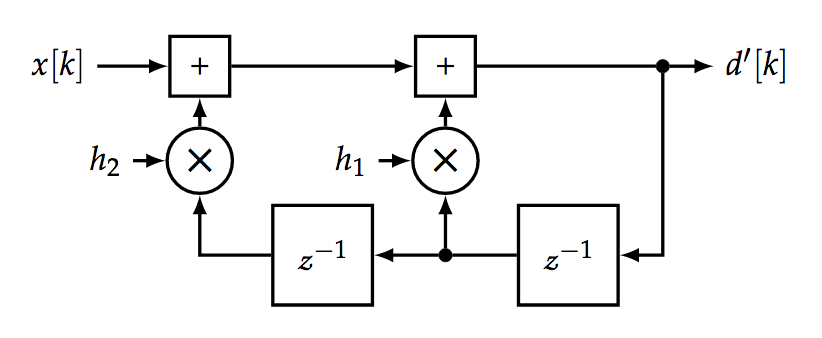
\includegraphics[width=0.5\textwidth]{figures/IIR_System.png}
 \caption{Blockschaltbild des zu untersuchenden IIR Systems ($h_1 = 0.82, h_2 = -0.03$) \cite{aufgabenstellung}.}
	\label{fig:IIR_System}
\end{figure}



\subsection{Anzahl an Filterkoeffizienten}

Ähnlich zur Untersuchung des FIR Filters wurde eine unterschiedliche Anzahl an Filterkoeffizienten verwendet und seine Auswirkung auf das Verhalten der Algorithmen überprüft ($N \in \{1, 2, 5\}$).
Anders als beim FIR Filter fällt beim Betrachten der Legenden der Filterkoeffizientenverläufe auf, dass die idealen Filterkoeffizienten bei der korrekten Anzahl ($N = 2$) nicht bestimmt werden konnten.
Selbst eine höhere Anzahl an Filterkoeffizienten (siehe Abb. \ref{fig:iir_N5}) führt nicht dazu das die Filterkoeffizienten auf die korrekten Werte konvergieren.
In den Abbildungen \ref{fig:iir_N1} bis \ref{fig:iir_N5} jedoch zu beobachten, dass der quadratische Fehler mit einer steigenden Anzahl an Filterkoeffizienten zunehmen kleiner wird.
Während in Abbildung \ref{fig:iir_N1} der Wert bei $Squared Error \approx 1.9$ liegt, so ist der Wert bei $N = 5$ in Abbildung \ref{fig:iir_N5} auf ca. $0.25$ gesunken.


\begin{figure}[H]
  \centering
      \includegraphics[width=0.9\textwidth]{{{figures/IIR/N_1_var_0.001}}}
 \caption{Vergleich zwischen LMS und RLS mit je einem Filterkoeffizienten (N=1)}
	\label{fig:iir_N1}
\end{figure}

\begin{figure}[H]
  \centering
      \includegraphics[width=0.9\textwidth]{{{figures/IIR/N_2_var_0.001}}}
 \caption{Vergleich zwischen LMS und RLS mit je zwei Filterkoeffizienten (N=2)}
	\label{fig:iir_N2}
\end{figure}

\begin{figure}[H]
  \centering
      \includegraphics[width=0.9\textwidth]{{{figures/IIR/N_5_var_0.001}}}
 \caption{Vergleich zwischen LMS und RLS mit je fünf Filterkoeffizienten (N=5)}
	\label{fig:iir_N5}
\end{figure}




\subsection{Einfluss der Varianz}

Beim Betrachten des Einflusses der Varianz des hinzugefügten AWGN zeigen sich deutliche Parallelen zu den Ergebnissen aus Abschnitt \ref{sec:FIR_sigma} der Untersuchung des FIR Systems.
Auch hier bedeutet eine Zunahme der Varianz des hinzugefügten Rauschens eine Zunahme des quadratischen Fehlers.
Vergleicht man die Abbildung \ref{fig:sig1} mit \ref{fig:IIR_sig1} und \ref{fig:sig10} mit \ref{fig:IIR_sig10} so sieht man das der Fehler beim Untersuchen des IIR Filters leicht über den Werten für den Fehler des FIR Filters liegt.
Das Adaptionsverhalten der Filterkoeffizienten wird durch die höhere Varianz des Rauschen ebenfalls beeinflusst und führt zu einem unruhigeren Verlauf der Koeffizienten.
Den Algorithmen gelingt die Adaption für das IIR System also leicht schlechter als für das FIR System.


\begin{figure}[H]
  \centering
      \includegraphics[width=0.9\textwidth]{{{figures/IIR/N_5_var_1.0}}}
 \caption{Vergleich zwischen LMS und RLS bei einem AWGN von $\sigma^2 = 1$  (N=5)}
	\label{fig:IIR_sig1}
\end{figure}

\begin{figure}[H]
  \centering
      \includegraphics[width=0.9\textwidth]{{{figures/IIR/N_5_var_10.0}}}
 \caption{Vergleich zwischen LMS und RLS bei einem AWGN von $\sigma^2 = 10$  (N=5)}
	\label{fig:IIR_sig10}
\end{figure}


\subsection{Einfluss des Schrittweite \boldmath{$\mu$} und des Vergessensfaktors \boldmath{$\rho$}}

Da die Schrittweite $\mu$ und der Vergessensfaktors $\rho$ Eigenschaften des LMS respektive des RLS Algorithmus sind und nicht Eigenschaften des zu untersuchenden Systems, sind die Einflüsse dieser Parameter identisch zu deren Beschreibung in Abschnitt \ref{sec:FIR_mu} und \ref{sec:FIR_rho} der Untersuchung des FIR Systems.


\subsection{Wahl des Lernalgorithmus}

Die korrekten Werte der Koeffizienten des untersuchten Systems konnte weder mit dem LMS noch dem RLS unter Verwendung verschiedener Parameter berechnet werden.
Die berechneten Koeffizienten beider Algorithmen konvergieren nicht auf die vorgegebenen Werte und können das System nicht hinreichend genau approximiert.
Es ist zu beachten, dass es unter idealen Bedingungen (kein Rauschen, korrekte Parameter etc.) möglich ist die Koeffizienten eines FIR Systems mithilfe des LMS und RLS Algorithmus perfekt nachzubilden.
Dies wurde, wie in Abschnitt \ref{sec:iir} beschrieben, approximiert.
Bei einem IIR System ist dies jedoch mit den beiden untersuchten Algorithmen nicht exakt möglich, da IIR Systeme einen rekursiven Signalanteil besitzen, welcher weder im LMS noch im RLS Algorithmen abgebildet wird.
Auf Grundlage dessen ist mit den beiden Algorithmen nur eine Approximation des IIR Systems möglich.
Dies erklärt auch warum die exakten Filtergewichte aus \ref{fig:IIR_System} selbst bei einem hohen Wert für $N$ nicht erreicht werden.
Bei der Robustheit gegenüber Rauschen erweisen sich die Algorithmen als leicht anfälliger im Vergleich zur Untersuchung des FIR Systems.
Der RLS ist erneut leicht robuster gegenüber hinzugefügtem Rauschen verglichen mit dem LMS.





\section{Systemwechsel}
\label{sec:Systemwechsel}

Nun soll untersucht werden, wie gut die Algorithmen mit einem plötzlichen Systemwechsel umgehen können.
Dazu werden die gleichen Signale wie schon in Abschnitt \ref{sec:fir} und \ref{sec:iir} verwendet.
Nach 5000 Iterationen werden die Filterkoeffizienten des Systems geändert.
Es wird wie schon oben jeweils ein FIR und IIR System untersucht.
Da viele der Auswirkungen der verschiedenen Parametereinstellungen auf die Algorithmen in den vorhergehenden Abschnitten ausführlich behandelt wurden, werden in diesem Abschnitt nur die Einstellungen hervorgehoben, die das Adaptionsverhalten bei einem Systemwechsel besonders beeinflussen.
Besonderes Augenmerk wird dabei auf die Schrittweite $\mu$ und den Vergessensfaktor $\rho$ gelegt.


\subsection{Systemwechsel FIR System}

Zunächst betrachten wir den Systemwechsel im FIR System unter Benutzung der bisherigen Standardparameter ( $N = 5$, $\sigma^2 = 0.001$, $\mu = 0.01$, $\rho = 0.99$).

\begin{figure}[H]
  \centering
      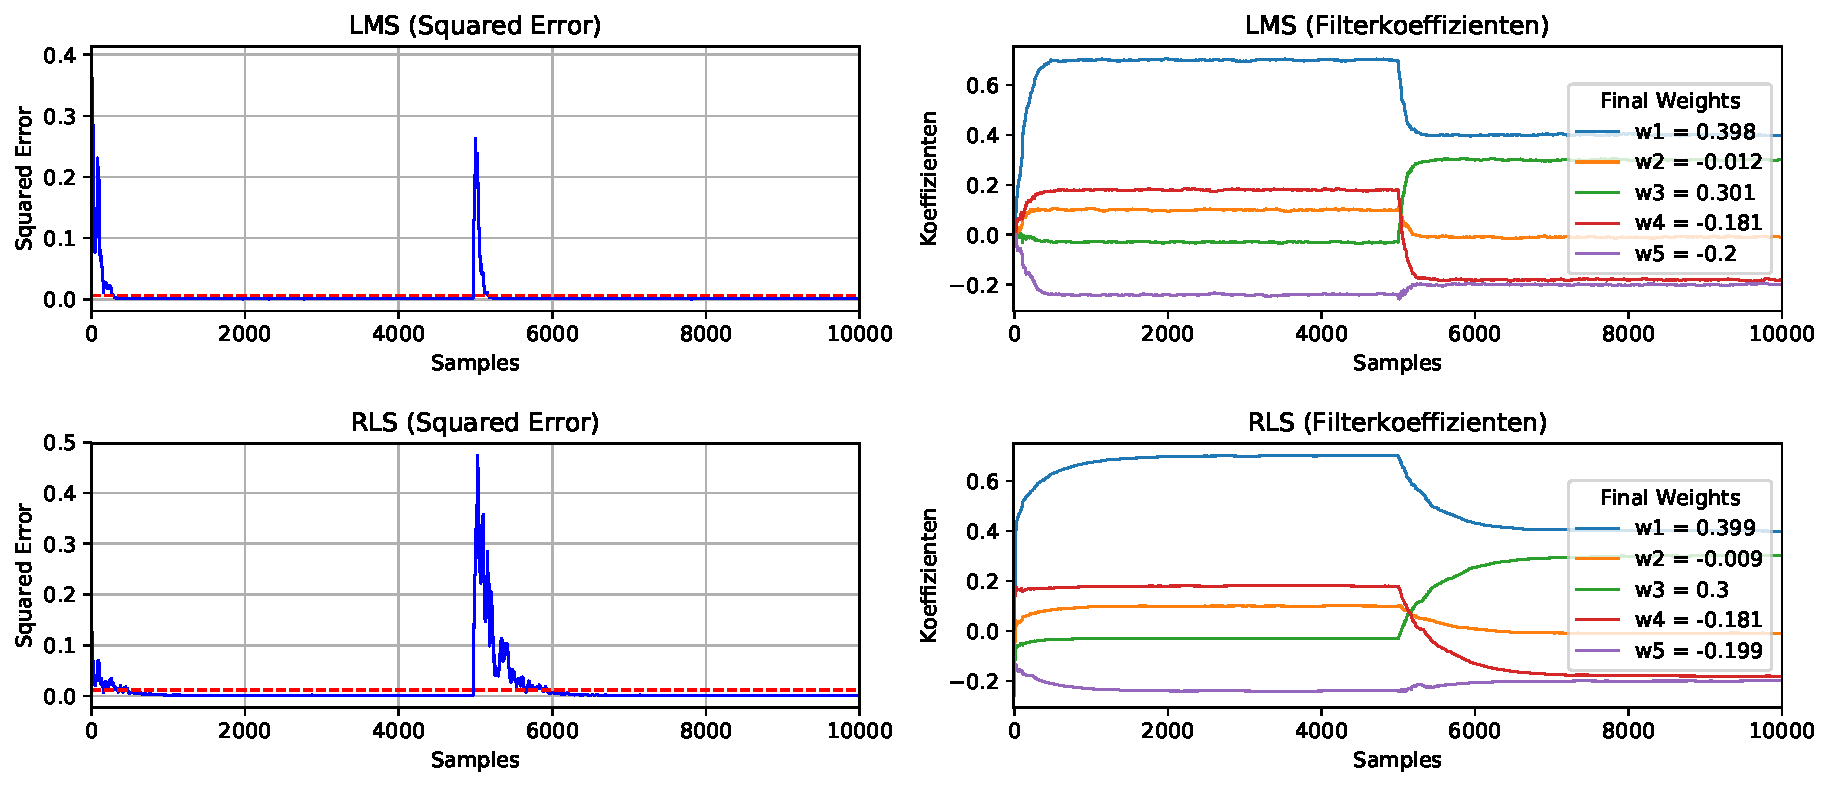
\includegraphics[width=0.9\textwidth]{{{figures/FIR_Systemwechsel/mu_0.01_rho_0.99}}}
 \caption{Systemwechsel im FIR System mit den bisherigen Standartparametern.}
	\label{fig:SW_FIR_1}
\end{figure}

Bei Betrachtung der Grafik \ref{fig:SW_FIR_1} ist der Systemwechsel nach 5000 Iterationen deutlich durch den sprunghaften Anstieg des quadratischen Fehlers und das Umschwenken der Filterkoeffizienten an dieser Stelle zu erkennen.
Es fällt auf das der quadratische Fehler des LMS kleiner ist als der des RLS und nach dem Systemwechsel deutlich schneller sinkt.
Der RLS kann sich wesentlich schlechter auf die neuen Werte des veränderten Systems einstellen. 
Dies wird besonders in den Plots der Koeffizientenverläufe sichtbar.
Während die Koeffizienten des LMS relativ sprunghaft nach dem Systemwechsel auf die neuen Koeffizienten konvergieren, so beschreiben die Filterkoeffizient des RLS ein deutlich längere nahezu exponentielle Kurve, bevor sie auf die neuen Filterwerte konvergieren.
Dies liegt an der Tatsache, das der RLS Algorithmus mehr vergangene Werte in die Berechnung der Filterkoeffizienten mit einbezieht als der LMS.


\begin{figure}[H]
  \centering
      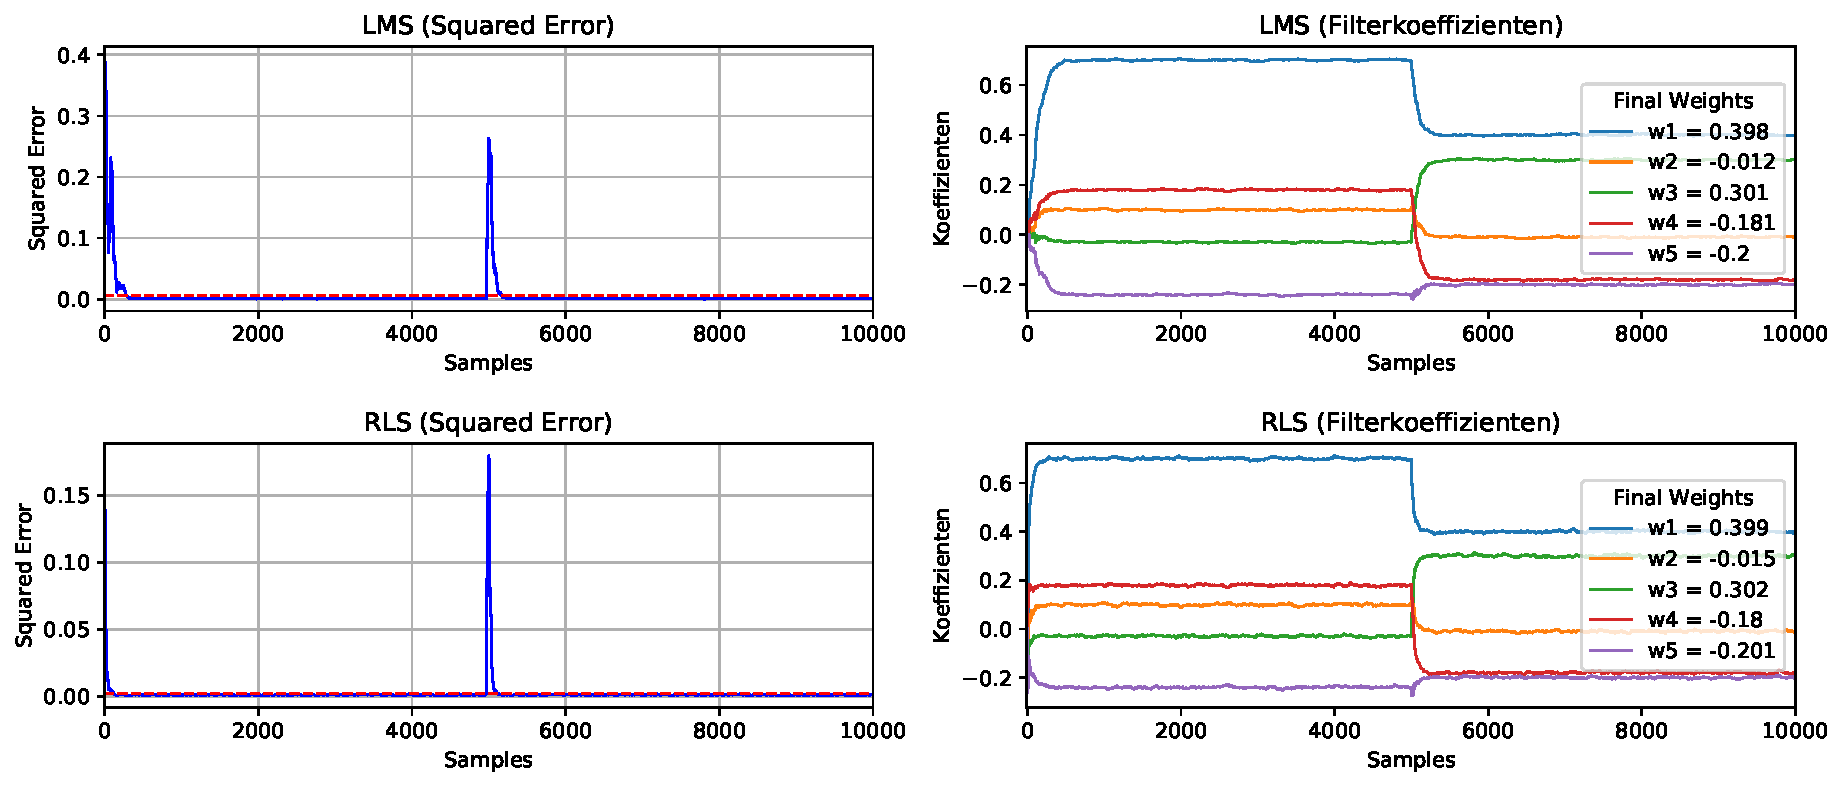
\includegraphics[width=0.9\textwidth]{{{figures/FIR_Systemwechsel/mu_0.01_rho_0.9}}}
 \caption{Systemwechsel im FIR System mit einem Vergessenfaktor von $\rho = 0.9$.}
	\label{fig:SW_FIR_2}
\end{figure}


Durch die Anpassung des Vergesensfaktors lässt sich das "`Gedächnis"' des KLS beeinflussen und einstellen wie stark die bisherigen Werte in der Berechnung gewichtet werden.
In Abbildung \ref{fig:SW_FIR_2} wurde der Vergessensfakor $\rho$ auf $0.9$ gesetzt.
Der quadratische Fehler des RLS sinkt dadurch erheblich schneller als zuvor und bleibt sogar unter dem Wert des LMS.
Auch die Filterkoeffizienten des RLS passen sich nun ähnlich schnell an wie die des LMS.
Es ist allerdings zu beobachten, dass die Filterkoeffizienten leicht oszillieren und nicht so sauber auf die korrekten Koeffizienten des Systems konvergieren.
Wird der Vergessensfaktor $\rho$ noch kleiner gesetzt, so verstärkt sich dieser Effekt weiter.

Gleiches gilt für die Schrittweite $\mu$ des LMS.
Wird diese auf einen höheren Wert gesetzt (z.B.: $0.2$) so verringert sich ebenfalls die Konvergenzzeit, jedoch wird das "`Rauschen"' im Verlauf der Filterkoeffizienten stärker und die Werte konvergieren nicht mehr auf die optimalen Ergebnisse.
Durch ein geschicktes Wählen der Schrittweite und des Vergessensfaktors lassen sich mit beiden Algorithmen annährend identische Ergebnisse erzielen.
Die ist im Abbildung \ref{fig:SW_FIR_3} zu sehen.
Dort wurde eine Schrittweite von $\mu = 0.03$ und ein Vergessensfaktor von $\rho = 0.9$ gewählt.


\begin{figure}[H]
  \centering
      \includegraphics[width=0.9\textwidth]{{{figures/FIR_Systemwechsel/mu_0.03_rho_0.9}}}
 \caption{Systemwechsel im FIR System mit einem Vergessensfaktor von $\rho = 0.9$ und einer Schrittweite von $\mu = 0.03$.}
	\label{fig:SW_FIR_3}
\end{figure}



\subsection{Systemwechsel IIR System}

Der Systemwechsel beim IIR System wird mit den selben Werten wie die anderen Abbildungen aus Abschnitt \ref{sec:fir} untersucht ($N =5$, $\sigma^2 = 0.01$).
Für die Parameter der Schrittweite und des Vergessensfaktors treffen auch die selben Erkenntnisse zu wie beim Systemwechsel des FIR Systems.
Durch eine zu große Schrittweite über- bzw. unterschreitet der LMS die optimalen Filterkoeffizienten periodisch und findet so nie die optimalen Werte.
Der Vergessensfaktor beeinflusst wie in den vorherigen Untersuchungen die Geschwindigkeit des Konvergierens und die Störanfälligkeit des RLS.
Werden die Parameter auf $\mu = 0.03$ für die Schrittweite und auf $\rho = 0.9$ für den Vergessenfaktor gesetzt, lassen sich wieder annährend identische Ergebnisse für die beiden Algorithmen erzielen (siehe \ref{fig:SW_IIR_1}).
Jedoch gilt für den ersten Teil des Signals vor dem Systemwechsel, wie schon in Abschnitt \ref{sec:iir}, dass das IIR System mit den beiden verwendeten Algorithmen nicht perfekt nachgebildet werden kann, da die Algorithmen im Unterschied zum IIR System keinen rekursiven Anteil haben.
Das zweite System scheint keinen oder nur einen sehr gering gewichteten rekursiv Teil zu haben, da der Fehler beider Algorithmen gegen 0 konvergiert.

\begin{figure}[H]
  \centering
      \includegraphics[width=0.9\textwidth]{{{figures/IIR_Systemwechsel/mu_0.03_rho_0.9}}}
 \caption{Systemwechsel im IIR System mit einem Vergessensfaktor von $\rho = 0.9$ und einer Schrittweite von $\mu = 0.03$.}
	\label{fig:SW_IIR_1}
\end{figure}



\subsection{Ergebnis}

In seiner Grundeinstellung eignet sich der LMS Algorithmus besser um trotz eines Systemwechsels innerhalb einer sehr kurzen Adaptionszeit gute Ergebnisse für die Filterkoeffizienten zu liefern.
Dies liegt an der Struktur des LMS, da er für seine Berechnung nur eine kleine Menge ($N$) an vergangenen Werte berücksichtigt.
Dadurch kann er schneller auf ein sich veränderndes System reagieren.
Während das Miteinbeziehen aller vorheriger Werte durch den RLS in den vorherigen Systemidentifikationen von statischen Systemen vorteilhaft war und zu einer extrem kurzen Konvergenzzeit geführt hat, wird diese Eigenschaft bei einem Systemwechsel zu einem Nachteil, weil der Algorithmus nicht schnell genug auf die Änderungen reagieren kann.
Dies kann durch das richtige Einstellen des Vergessensfaktors behoben werden und dem RLS ebenfalls zu einer schnellen Konvergenzzeit nach dem Systemwechsel verhelfen.
Wie aus den Plots \ref{fig:SW_FIR_3} und \ref{fig:SW_IIR_1} hervorgeht bedeutet dies, dass bei einer korrekten Wahl der jeweiligen Parameter keiner der beiden Algorithmen dem Anderen überlegen ist.
Bei beiden Algorithmen ist zu berücksichtigen, dass die Einstellung des Vergessensfaktors bzw. der Schrittweite immer einen Trade-off zwischen der Konvergenzzeit und der Stabilität des Verlaufs der Koeffizienten darstellt.





\section{Kernel Least Mean Squares Algorithmus}
\label{sec:klms}

In diesem Abschnitt wird ein dritter Algorithmus, der Kernel Least Mean Squares (KLMS) untersucht.
Er nimmt eine Zeitreihenschätzung vor und approximiert die Filterkoeffizienten des unbekannten Systems mit Hilfe eines Trainingsdatensatzes.
Der in der Aufgabenstellung zur Verfügung gestellte Trainingsdatensatz ($Training.mat$) umfasst 500 Werte.
Die Performance der auf dem Trainingsdatensatz trainierten Filter wird mit einer Testdatenreihe ($Test.mat$) von 10000 Werten untersucht.
Anschließend sollen die trainierten Filter mit den Ergebnissen des LMS verglichen werden.


\subsection{Filterentwurf}

Zwei unterschiedliche Filter wurden trainiert, einmal mit 5 (siehe Abbildung \ref{fig:klms5}) und einmal 10 (siehe Abbildung \ref{fig:klms10}) Filterkoeffizienten.
Die Parameter $\mu$ und $\sigma$ wurden frei gewählt.
Die vorgestellten Ergebnisse der KLMS Filter wurden auf Basis eines Gauss-Kernels erstellt.
Es ist auch möglich alternativ andere Kernel  zu wählen (z.B. Laplace-Kernel).


\begin{figure}[H]
  \centering
      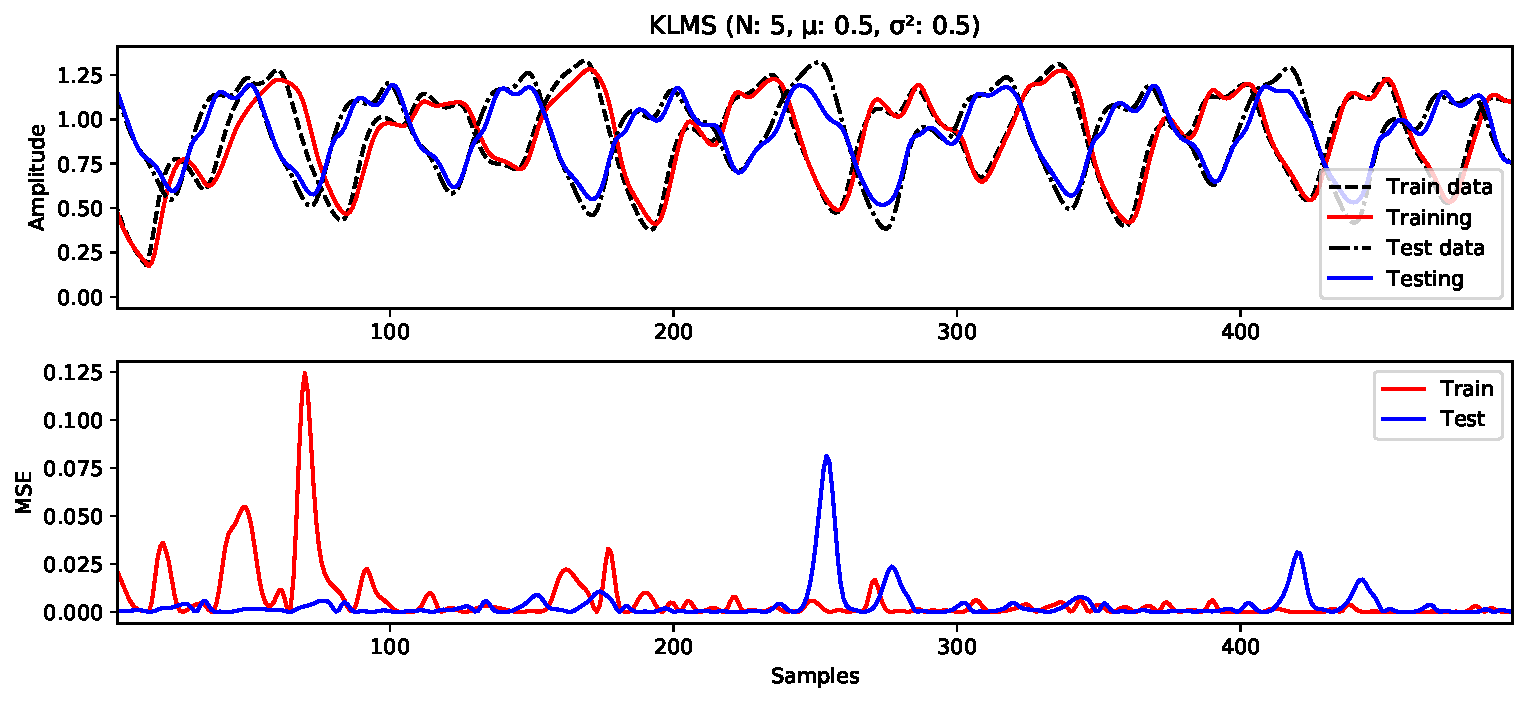
\includegraphics[width=0.7\textwidth]{{{figures/KLMS_5_0.5_0.5_kernel_weights}}}
  \caption{Training und Test mit KLMS und 5 Filterkoeffizienten}
  \label{fig:klms5}
\end{figure}

\begin{figure}[H]
  \centering
      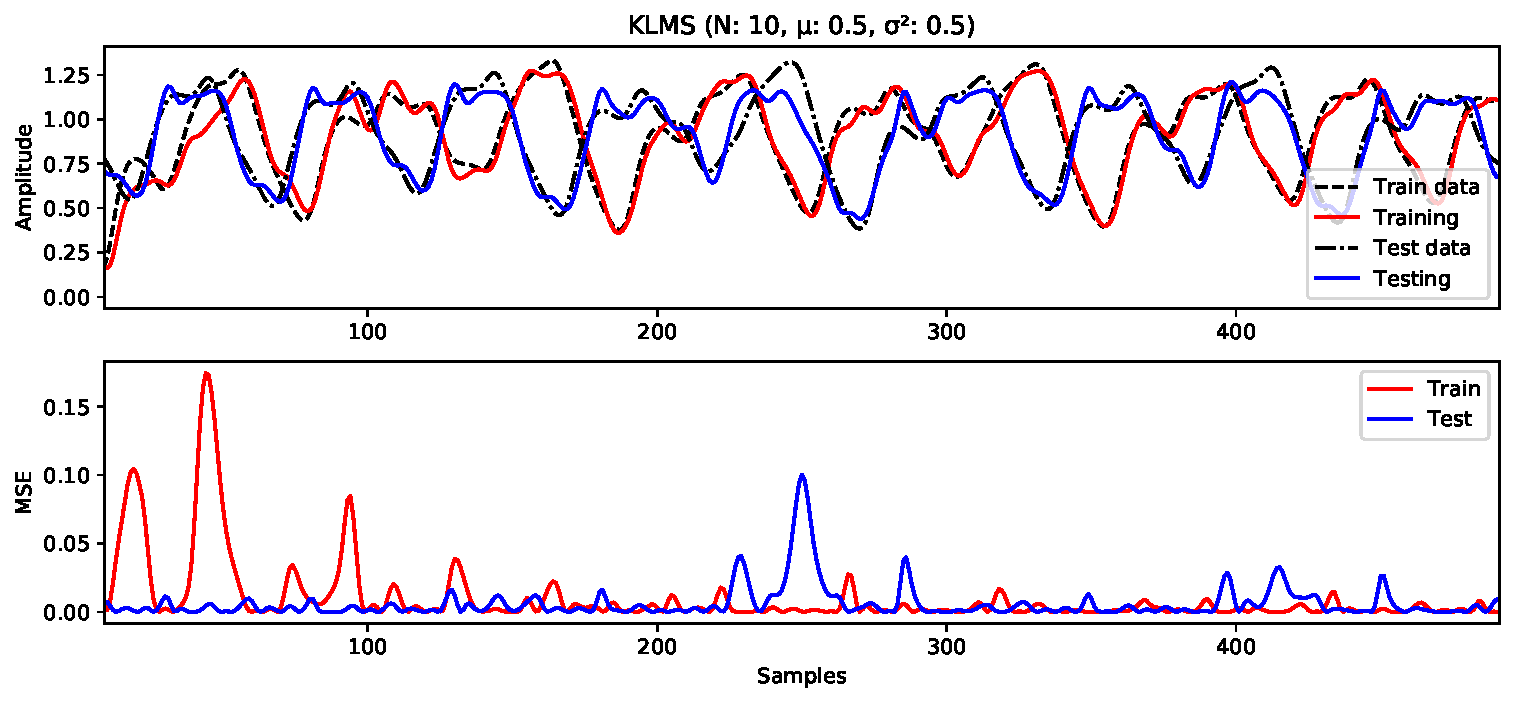
\includegraphics[width=0.7\textwidth]{{{figures/KLMS_10_0.5_0.5_kernel_weights}}}
  \caption{Training und Test mit KLMS und 10 Filterkoeffizienten}
  \label{fig:klms10}
\end{figure}


Es fällt auf, dass die trainierten Filter im Trainingsdurchlauf einen kleineren Fehler aufweisen als im Testdurchlauf.
Mit diesem Verhalten war zu rechnen, da sich die Systeme im Lernprozess systematisch anpassen.
Die Wahl der Parameter $\mu$ und $\sigma$ wurde über mehrere Iterationen verfeinert.
Dabei hatte die Breite der Gauss-Kerne durch die Varianz $\sigma$ einen ebenso wichtigen Einfluss wie die Schrittweite $\mu$.
Schließlich wurde für $\mu = 0.5$ und $\sigma = 0.5$ gewählt, womit die Filter ein zufriedenstellendes Adaptionsverhalten aufwiesen.
Bei einer tiefgehenderen Untersuchung der Systeme könnte mit Hilfe einer Crossvalidierung versucht werden, die optimalen $\mu$ und $\sigma$ Parameter zu ermitteln.


\subsection{Vergleich von KLMS und LMS}
Es wurden ein LMS System auf Grundlage der Trainingsdaten erstellt.
Die Filtergewichtung der Systeme wurden anschließend eingefroren und im darauffolgenden Testdurchlauf auf dem Testdatensatz nicht weiter angepasst.
Dadurch konnte ein objektiver Vergleich zwischen den Algorithmen vorgenommen werden.



